\documentclass[12pt,letterpaper]{article}

% --- Preamble (shared with main manuscript) ---
% manuscript-preamble.tex — Chicago Author-Date manuscript preamble
% Shared preamble for manuscript and potential slide reuse

% --- Fonts ---
% Support both PdfLaTeX and Xe/LuaLaTeX.
\usepackage{iftex}
\ifPDFTeX
  \usepackage[T1]{fontenc}
  \usepackage[utf8]{inputenc}
  \usepackage{newtxtext}
  \usepackage{newtxmath}
\else
  \usepackage{fontspec}
  \setmainfont{Times New Roman}[Ligatures=TeX]
\fi

% --- Layout ---
\usepackage[margin=1in]{geometry}
\usepackage{setspace}
\doublespacing

% --- Math & symbols ---
\usepackage{amsmath}
\ifPDFTeX
  % newtxmath already provides most AMS-style symbols under PdfLaTeX
\else
  \usepackage{amssymb}
\fi

% --- Tables ---
\usepackage{booktabs}
\usepackage{tabularx}
\usepackage{longtable}
\usepackage{multirow}
\usepackage{array}
\usepackage{dcolumn}

% --- Figures ---
\usepackage{graphicx}
\usepackage{float}

% --- Citations (Chicago Author-Date via biblatex-chicago) ---
% Compile: xelatex -> biber -> xelatex -> xelatex
\usepackage[
  authordate,
  backend=biber,
  natbib=true,
  url=true,
  doi=true,
  isbn=false
]{biblatex-chicago}
\addbibresource{references.bib}

% --- Cross-references & links ---
\usepackage{hyperref}
\hypersetup{
  colorlinks=true,
  linkcolor=black,
  citecolor=black,
  urlcolor=blue,
  pdfauthor={},
  pdftitle={Issue-Bounded Conditionality in U.S. Public Opinion on Fentanyl Policy}
}

% --- Appendix support ---
\usepackage[toc,page]{appendix}

% --- Landscape pages for wide tables ---
\usepackage{pdflscape}

% --- Misc ---
\usepackage{enumerate}
\usepackage{etoolbox}
\usepackage{caption}
\captionsetup{font=small,labelfont=bf,hypcap=false}

% --- Prevent doublespacing inside tables ---
\AtBeginEnvironment{tabular}{\singlespacing}
\AtBeginEnvironment{longtable}{\singlespacing}

% --- Reduce noisy line-breaking diagnostics ---
\hbadness=10000
\hfuzz=200pt


\vbadness=10000
\vfuzz=500pt


% --- Metadata ---
\title{Online Supplementary Material\\
\large When Warm Feelings Harden: Fentanyl Crisis Blame and U.S.\ Public Opinion on China}
\author{Junyang Hu}
\date{\today}

\begin{document}

\maketitle
\thispagestyle{empty}

\noindent This online supplement contains robustness checks and supporting analyses referenced in the main article. Tables and figures are numbered with an ``A'' prefix and correspond to the references in the main text.

\newpage
\setcounter{page}{1}

\appendix
\renewcommand{\thetable}{A\arabic{table}}
\setcounter{table}{0}
\renewcommand{\thefigure}{A\arabic{figure}}
\setcounter{figure}{0}

\section{Supplementary Tables and Figures}
\label{sec:appendix}

% --- Phase 3 Appendix ---
\subsection{Robustness: Alternative Blame Measure and Ordinal Models}

Table~\ref{tab:phase3_panel_b} (in the main text) replicates the posture models using \texttt{blame\_china\_alt}, the single-choice ``most responsible'' item. The warmth $\times$ blame interaction is attenuated but retains the expected sign.

\begin{table}[htbp]
\centering
\small
\caption{Robustness: Ordinal Logit on Individual Posture Items}
\label{tab:app_olr}

\begin{tabular}[t]{lllll}
\toprule
Item & Wave & Warmth (b/SE/p) & Blame (b/SE/p) & Interaction (b/SE/p)\\
\midrule
Defensive (a) & 2024 & 0.345 (0.073) 0.000*** & -0.172 (0.085) 0.042* & 0.324 (0.097) 0.001***\\
Defensive (a) & 2025 & 0.349 (0.095) 0.000*** & -0.247 (0.115) 0.032* & 0.462 (0.126) 0.000***\\
Defensive (a) & Pooled & 0.342 (0.057) 0.000*** & -0.197 (0.068) 0.004** & 0.379 (0.076) 0.000***\\
Cooperative (b) & 2024 & 0.703 (0.076) 0.000*** & -0.230 (0.089) 0.010** & 0.078 (0.110) 0.480\\
Cooperative (b) & 2025 & 0.638 (0.095) 0.000*** & -0.322 (0.109) 0.003** & 0.260 (0.122) 0.033*\\
Cooperative (b) & Pooled & 0.672 (0.059) 0.000*** & -0.256 (0.067) 0.000*** & 0.151 (0.081) 0.063\\
Friendly (c, rev.) & 2024 & 0.749 (0.073) 0.000*** & 0.082 (0.088) 0.353 & 0.210 (0.099) 0.034*\\
Friendly (c, rev.) & 2025 & 0.500 (0.097) 0.000*** & -0.009 (0.104) 0.935 & 0.284 (0.123) 0.020*\\
Friendly (c, rev.) & Pooled & 0.639 (0.058) 0.000*** & 0.044 (0.067) 0.513 & 0.245 (0.077) 0.001**\\
Constructive (d) & 2024 & 0.557 (0.070) 0.000*** & 0.088 (0.089) 0.319 & 0.096 (0.103) 0.347\\
Constructive (d) & 2025 & 0.493 (0.092) 0.000*** & 0.142 (0.107) 0.184 & 0.126 (0.118) 0.287\\
Constructive (d) & Pooled & 0.521 (0.056) 0.000*** & 0.115 (0.066) 0.083 & 0.114 (0.076) 0.133\\
\bottomrule
\end{tabular}

\par\vspace{0.5ex}
{\footnotesize\textit{Notes.} Survey-weighted ordinal logistic regressions (\texttt{svyolr}). Each row reports a separate model for one of four posture items (scale 1--5). Coefficients reflect the log-odds of a higher response. Standard errors are design-based. $n$ is unweighted. * $p<0.10$, ** $p<0.05$, *** $p<0.01$.}
\end{table}

Table~\ref{tab:phase3_r1} reports replacement robustness models substituting the behavior index for blame in the interaction term.

\begin{table}[htbp]
\centering
\small
\caption{Robustness: Behavior Index in Place of Blame}
\label{tab:phase3_r1}

\begin{table}[htbp]
\begin{center}
\begin{tabular}{l c c}
\hline
 & R1: blame\_china & R1: blame\_china\_alt \\
\hline
(Intercept)                          & $0.50^{***}$  & $0.50^{***}$  \\
                                     & $(0.08)$      & $(0.09)$      \\
behavior\_index\_z                   & $0.34^{***}$  & $0.40^{***}$  \\
                                     & $(0.03)$      & $(0.02)$      \\
blame\_china                         & $-0.07^{*}$   &               \\
                                     & $(0.03)$      &               \\
factor(year)2025                     & $0.14^{***}$  & $0.15^{***}$  \\
                                     & $(0.03)$      & $(0.03)$      \\
party3Republican                     & $-0.08$       & $-0.06$       \\
                                     & $(0.05)$      & $(0.05)$      \\
party3Independent                    & $0.01$        & $0.02$        \\
                                     & $(0.04)$      & $(0.04)$      \\
ideo5\_clean                         & $-0.10^{***}$ & $-0.11^{***}$ \\
                                     & $(0.02)$      & $(0.02)$      \\
educ\_college                        & $-0.00$       & $0.01$        \\
                                     & $(0.03)$      & $(0.03)$      \\
age                                  & $-0.00^{***}$ & $-0.00^{***}$ \\
                                     & $(0.00)$      & $(0.00)$      \\
female                               & $0.05$        & $0.05$        \\
                                     & $(0.03)$      & $(0.03)$      \\
race\_ethBlack                       & $0.02$        & $0.04$        \\
                                     & $(0.05)$      & $(0.05)$      \\
race\_ethHispanic                    & $0.04$        & $0.03$        \\
                                     & $(0.06)$      & $(0.06)$      \\
race\_ethAsian                       & $-0.16$       & $-0.15$       \\
                                     & $(0.09)$      & $(0.09)$      \\
race\_ethOther                       & $0.02$        & $0.04$        \\
                                     & $(0.05)$      & $(0.06)$      \\
newsint\_attn                        & $0.01$        & $0.01$        \\
                                     & $(0.02)$      & $(0.02)$      \\
exposure\_index                      & $-0.00$       & $0.00$        \\
                                     & $(0.03)$      & $(0.03)$      \\
behavior\_index\_z:blame\_china      & $0.14^{***}$  &               \\
                                     & $(0.03)$      &               \\
blame\_china\_alt                    &               & $-0.16^{***}$ \\
                                     &               & $(0.05)$      \\
behavior\_index\_z:blame\_china\_alt &               & $0.07$        \\
                                     &               & $(0.05)$      \\
\hline
Deviance                             & $3095.58$     & $2935.01$     \\
Dispersion                           & $0.73$        & $0.73$        \\
Num. obs.                            & $4234$        & $4026$        \\
\hline
\multicolumn{3}{l}{\scriptsize{$^{***}p<0.001$; $^{**}p<0.01$; $^{*}p<0.05$}}
\end{tabular}
\caption{Replacement Robustness: Behavior Index $\times$ Blame (Pooled)}
\label{tab:phase3_r1}
\end{center}
\end{table}

\par\vspace{0.5ex}
{\footnotesize\textit{Notes.} Survey-weighted OLS. Dependent variable: standardized foreign-policy posture index (\texttt{posture\_z}). Columns substitute the behavior index (\texttt{behavior\_index\_z}) for the binary blame variable as the conditioning variable. Standard errors are design-based. * $p<0.05$, ** $p<0.01$, *** $p<0.001$.}
\end{table}

% --- Acquiescence and Full Coefficients ---
\subsection{Robustness: Acquiescence and Full Coefficients}

Acquiescence-controlled estimates of the blame effect on $\hat{P}(\text{S+A})$ are reported in Table~\ref{tab:app_acquiescence}.

\begin{table}[htbp]
\centering
\small
\caption{Acquiescence-Adjusted Blame Effects: With and Without Endorsement-Count Control}
\label{tab:app_acquiescence}
\begin{table}[!h]
\centering
\caption{Acquiescence Robustness: Blame Effect on P(S+A) With/Without Endorsement Controls}
\label{tab:app_acquiescence}
\centering
\begin{tabular}[t]{lrr}
\toprule
variant & Dpp\_SA(w=-1) & Dpp\_SA(w=+1)\\
\midrule
Baseline & 0.2944301 & 0.3058172\\
+ main + miss & 0.2111030 & 0.1910461\\
+ zero-imputed & 0.2111030 & 0.1910461\\
\bottomrule
\end{tabular}
\end{table}

\par\vspace{0.5ex}
{\footnotesize\textit{Notes.} Survey-weighted multinomial logit marginal effects. Each row reports the blame-driven shift in $\hat{P}(\text{S+A})$ at the indicated warmth level, with and without endorsement-count control for acquiescent response style. The endorsement-count covariate is the count of items the respondent endorsed across the broader policy-tool checklist, \emph{excluding} the two items (sanctions, action) that define the S+A tool configuration to avoid mechanical correlation with the dependent variable; counts are computed within wave from the items shared across both 2024 and 2025 instruments. Higher values indicate a stronger general tendency to endorse listed items independent of any specific position on China policy. The endorsement-count control attenuates the blame effect on $P(\text{S+A})$ by approximately 38\%.}
\end{table}

\begin{table}[htbp]
\centering
\small
\caption{Design-Based Sensitivity Check: MNL S+A Coefficients (Log-Odds Scale)}
\label{tab:app_design_mnl}

\begin{tabular}[t]{llrrrrl}
\toprule
Outcome & Predictor & Estimate & Design SE & t-value & p-value & Stars\\
\midrule
Sanctions-only & warmth\_z & 0.0474 & 0.0619 & 0.766 & 0.4439 & \\
Action-only & warmth\_z & 0.0632 & 0.1016 & 0.622 & 0.5342 & \\
S+A & warmth\_z & -0.2269 & 0.1018 & -2.228 & 0.0259 & *\\
Sanctions-only & blame\_china & 0.8045 & 0.0927 & 8.676 & 0.0000 & ***\\
Action-only & blame\_china & 1.6519 & 0.1314 & 12.572 & 0.0000 & ***\\
S+A & blame\_china & 2.6398 & 0.1130 & 23.353 & 0.0000 & ***\\
Sanctions-only & factor(year)2025 & -0.2426 & 0.0871 & -2.785 & 0.0054 & **\\
Action-only & factor(year)2025 & -0.0559 & 0.1191 & -0.469 & 0.6391 & \\
S+A & factor(year)2025 & -0.1267 & 0.0922 & -1.373 & 0.1697 & \\
Sanctions-only & warmth\_z:blame\_china & -0.1927 & 0.0894 & -2.154 & 0.0313 & *\\
Action-only & warmth\_z:blame\_china & -0.1546 & 0.1257 & -1.230 & 0.2189 & \\
S+A & warmth\_z:blame\_china & 0.1343 & 0.1143 & 1.175 & 0.2402 & \\
\bottomrule
\end{tabular}

\par\vspace{0.5ex}
{\footnotesize\textit{Notes.} Design-based standard errors computed via \texttt{svyglm()} binary contrasts (S+A vs.\ all other categories) on the log-odds scale. The binary-contrast approach approximates the design-based equivalent of the full MNL. Point estimates are consistent with the main multinomial specification. The blame main effect on S+A is robust ($b = 2.640$, $p < 0.001$); the warmth $\times$ blame interaction is not statistically distinguishable from zero under design-based inference ($b = 0.134$, $p = 0.240$).}
\end{table}

\begin{figure}[htbp]
  \centering
  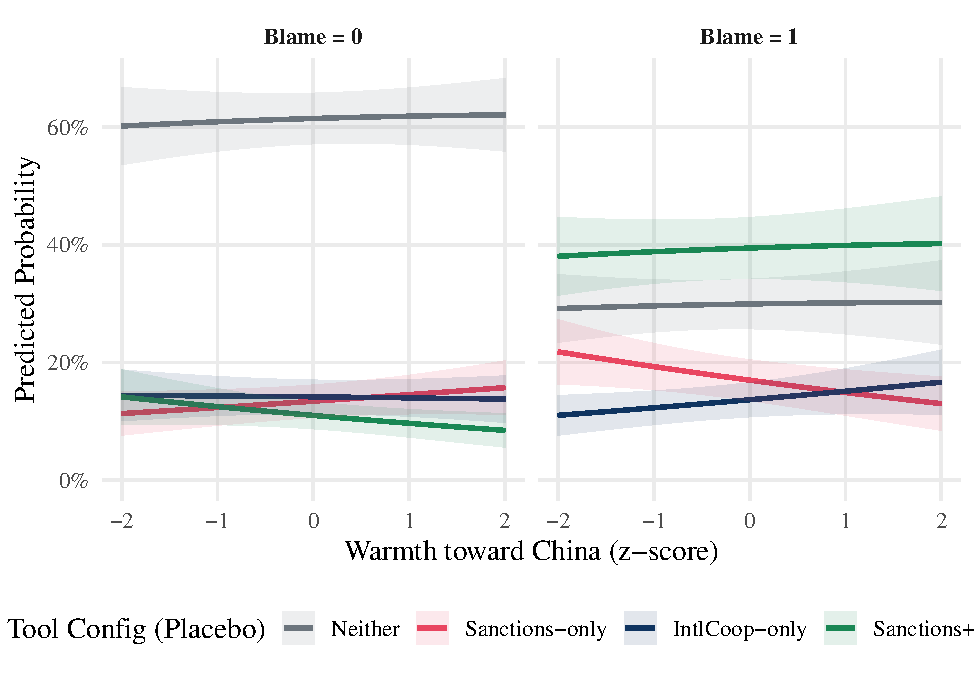
\includegraphics[width=0.85\textwidth]{figures/app_fig_placebo_sanctionsXintlcoop.pdf}
  \caption{Placebo test: Interaction plot for sanctions $\times$ international cooperation composite as dependent variable. The placebo pairing shows a comparable blame-driven shift ($\Delta_{\text{pp}} = 0.311$ at warmth $= +1$\,SD), indicating that the S+A effect is not fully specific to fentanyl cooperation.}
  \label{fig:app_placebo}
\end{figure}

% --- Phase 5 Appendix ---
\subsection{Robustness: Full Panorama, Pairwise Divergence, and Alternative Specifications}

\begin{table}[htbp]
\centering
\small
\caption{Eight-Probe Panorama: S+A Minus Sanctions-Only Contrasts Across All Scenarios}
\label{tab:app_panorama}
\footnotesize

\begin{tabular}[t]{llllll}
\toprule
Probe & Domain & Estimate & SE & CI & p\_value\\
\midrule
a: Taiwan military action & Security & -0.0750 & 0.0688 & {}[-0.2099, 0.0599] & 0.276\\
b: US-China military collision & Security & 0.0285 & 0.0826 & {}[-0.1335, 0.1905] & 0.730\\
c: Other military collision & Security & 0.0728 & 0.0734 & {}[-0.0711, 0.2168] & 0.321\\
d: Fentanyl cooperation & Health & 0.2817 & 0.0913 & {}[0.1027, 0.4607] & 0.002**\\
e: Resuming adoptions & Cultural & 0.0837 & 0.0872 & {}[-0.0873, 0.2547] & 0.337\\
f: Electronics sales stopped & Economic & 0.1257 & 0.0916 & {}[-0.0540, 0.3053] & 0.170\\
g: Student scholarships & Cultural & 0.0160 & 0.0882 & {}[-0.1570, 0.1891] & 0.856\\
h: Pandas to US zoos & Cultural & 0.0402 & 0.0769 & {}[-0.1106, 0.1911] & 0.601\\
\bottomrule
\end{tabular}

\par\vspace{0.5ex}
{\footnotesize\textit{Notes.} Survey-weighted stacked OLS. Each row reports the blame-driven S+A minus Sanctions-only contrast ($\Delta_s$) for one of eight probes, among warm respondents ($\texttt{warmth\_z} = +1$\,SD). Standard errors are clustered at the respondent level. 95\% confidence intervals reported. $p$-values are two-sided.}
\end{table}

\begin{table}[htbp]
\centering
\small
\caption{Pairwise Divergence Tests: Target Probe vs.\ Boundary Probes (BH-FDR Corrected)}
\label{tab:app_divergence}

\begin{tabular}[t]{llllll}
\toprule
Comparison & Divergence & SE & CI & p\_value & p\_fdr\\
\midrule
d vs a: Taiwan military action & 0.3567 & 0.1200 & {}[0.1213, 0.5921] & 0.003** & 0.021*\\
d vs b: US-China military collision & 0.2532 & 0.1208 & {}[0.0163, 0.4902] & 0.036* & 0.063\\
d vs c: Other military collision & 0.2089 & 0.1122 & {}[-0.0111, 0.4289] & 0.063 & 0.088\\
d vs e: Resuming adoptions & 0.1980 & 0.1117 & {}[-0.0210, 0.4170] & 0.076 & 0.089\\
d vs f: Electronics sales stopped & 0.1560 & 0.1202 & {}[-0.0798, 0.3919] & 0.195 & 0.195\\
d vs g: Student scholarships & 0.2657 & 0.1048 & {}[0.0601, 0.4712] & 0.011* & 0.040*\\
d vs h: Pandas to US zoos & 0.2415 & 0.1089 & {}[0.0279, 0.4550] & 0.027* & 0.062\\
\bottomrule
\end{tabular}

\par\vspace{0.5ex}
{\footnotesize\textit{Notes.} Each row reports a pairwise contrast between $\Delta_d$ (probe $d$, fentanyl cooperation) and one boundary probe. $p$-values are two-sided; $p_{\text{FDR}}$ applies the Benjamini--Hochberg false discovery rate correction across seven comparisons. Standard errors are clustered at the respondent level.}
\end{table}

\begin{table}[htbp]
\centering
\small
\caption{Alternative Specification: Continuous $\hat{P}(\text{S+A})$ as Dependent Variable}
\label{tab:app_phat}
\begin{table}[!h]
\centering
\caption{Phase 5 Appendix: P\_hat(S+A) Continuous Specification (probe d)}
\centering
\begin{tabular}[t]{lrrrrl}
\toprule
DV & Estimate & SE & t\_value & p\_value & Note\\
\midrule
probe\_d & 0.5018874 & 0.9951674 & 0.5043246 & 0.6140597 & SEs do not propagate Stage 1 uncertainty; directional only\\
\bottomrule
\end{tabular}
\end{table}

\par\vspace{0.5ex}
{\footnotesize\textit{Notes.} Blame-driven shifts in MNL-predicted $\hat{P}(\text{S+A})$ (continuous, replacing the binary S+A classifier). Compare to main estimates in Table~\ref{tab:phase5_contrasts}.}
\end{table}

\begin{figure}[htbp]
  \centering
  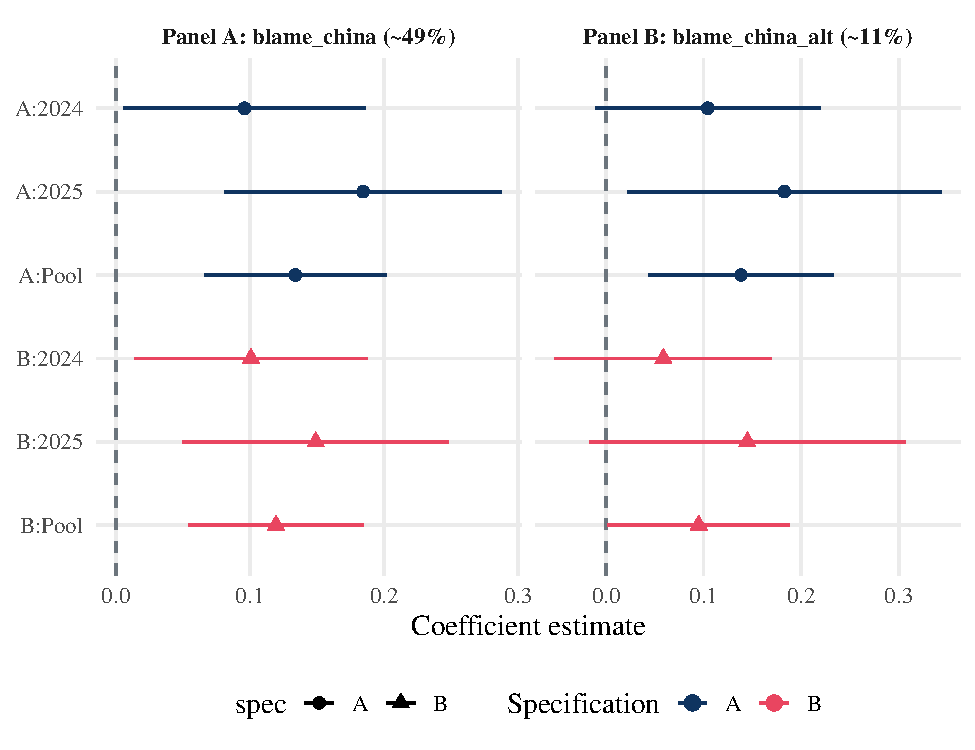
\includegraphics[width=0.85\textwidth]{figures/fig_coef_forest_interaction.pdf}
  \caption{Coefficient forest plot for the warmth $\times$ blame interaction across model specifications. Point estimates with 95\% confidence intervals.}
  \label{fig:app_forest}
\end{figure}

% --- Cross-Wave Robustness ---
\subsection{Cross-Wave Robustness: Interaction Stability Across Survey Years}
\label{sec:app_crosswave}

The pooled models in the main text include year fixed effects to account for mean-level differences across the 2024 and 2025 waves. Table~\ref{tab:app_within_wave} reports wave-specific estimates confirming that the warmth $\times$ blame interaction is statistically significant in both the 2024 and 2025 waves individually.

\begin{table}[htbp]
\centering
\small
\caption{Within-Wave Replication: Warmth $\times$ Blame Interaction by Survey Year}
\label{tab:app_within_wave}
\input{tables/app_tab_within_wave}
\par\vspace{0.5ex}
{\footnotesize\textit{Notes.} Survey-weighted OLS estimated separately for each wave and pooled with year fixed effects. The warmth $\times$ blame interaction is statistically significant in both waves individually ($b_{2024} = 0.096$, $p = 0.037$; $b_{2025} = 0.185$, $p < 0.001$). The 2025 coefficient is larger, consistent with the post-tariff political context heightening the conditional pattern.}
\end{table}

% --- NA-1: MNL Post-Treatment Sensitivity ---
\subsection{Post-Treatment Sensitivity: Total-Effect MNL Specification}
\label{sec:app_posttx}

The main multinomial logit specification controls for \texttt{posture\_z}, which is a post-treatment covariate with respect to warmth and blame. Conditioning on a post-treatment variable can, in principle, bias the estimated effect of the primary predictors by absorbing part of the treatment path. Table~\ref{tab:app_mnl_total_effect} compares the within-posture specification (\texttt{posture\_z} included) against a total-effect specification that omits \texttt{posture\_z} entirely. The blame-driven shift in $\hat{P}(\text{S+A})$ is $\Delta = 0.306$ ($SE = 0.029$) under the within-posture specification and $\Delta = 0.305$ ($SE = 0.028$) under the total-effect specification at warmth $= +1$ SD; the difference between the two contrasts is less than 0.001. Post-treatment conditioning does not materially alter the estimated blame effect on tool configuration, confirming that the within-posture estimates carry the same substantive interpretation as the total-effect estimates. Standard errors in this table are Hessian-based (model-based) and are not directly comparable to design-based standard errors reported in the main results.

\begin{table}[htbp]
\centering
\small
\caption{Post-Treatment Sensitivity: Within-Posture vs.\ Total-Effect MNL Specification}
\label{tab:app_mnl_total_effect}
\scriptsize

\begin{tabular}[t]{llll}
\toprule
Specification & Outcome & Warmth x Blame & SE (model-based)\\
\midrule
--- MNL Coefficients (Warmth x Blame interaction) --- &  &  & \\
Within-posture (posture\_z included) & Sanctions-only & -0.1927 & 0.0894\\
Total-effect (posture\_z excluded) & Sanctions-only & -0.2098 & 0.0893\\
Within-posture (posture\_z included) & Action-only & -0.1546 & 0.1257\\
Total-effect (posture\_z excluded) & Action-only & -0.1578 & 0.1254\\
Within-posture (posture\_z included) & S+A & 0.1343 & 0.1143\\
Total-effect (posture\_z excluded) & S+A & 0.1289 & 0.1142\\
--- Blame contrasts: Dpp(S+A) at warmth levels --- &  &  & \\
Within-posture (posture\_z included) & warmth\_z = -1 & 0.2944 (SE=0.0248) & (predicted prob contrast)\\
Total-effect (posture\_z excluded) & warmth\_z = -1 & 0.2938 (SE=0.0246) & (predicted prob contrast)\\
Within-posture (posture\_z included) & warmth\_z = +0 & 0.3019 (SE=0.0234) & (predicted prob contrast)\\
Total-effect (posture\_z excluded) & warmth\_z = +0 & 0.3018 (SE=0.0233) & (predicted prob contrast)\\
Within-posture (posture\_z included) & warmth\_z = +1 & 0.3058 (SE=0.0289) & (predicted prob contrast)\\
Total-effect (posture\_z excluded) & warmth\_z = +1 & 0.3051 (SE=0.0284) & (predicted prob contrast)\\
Note: MNL SEs are Hessian-based (model-based); not directly comparable to design-based SEs in main tables. &  &  & \\
\bottomrule
\end{tabular}

\par\vspace{0.5ex}
{\footnotesize\textit{Notes.} Each panel compares the within-posture specification (\texttt{posture\_z} included as a control) against the total-effect specification (\texttt{posture\_z} omitted). The upper panel reports MNL log-odds coefficients on the warmth $\times$ blame interaction; the lower panel reports predicted probability contrasts ($\Delta_{\text{pp}}$) for the S+A outcome at three warmth levels. Standard errors are Hessian-based (model-based) and are not directly comparable to design-based standard errors in the main tables. The reference category is Neither.}
\end{table}

% --- NA-2: Formal Placebo Contrast ---
\subsection{Formal Placebo Contrast: Main vs.\ Placebo Blame Effect}
\label{sec:app_placebo_contrast}

Section~\ref{sec:discussion} notes that the placebo MNL (using sanctions $\times$ international cooperation as the dependent variable) produces a blame-driven shift comparable in magnitude to the main specification. Table~\ref{tab:app_placebo_contrast} formalizes this comparison. The main blame contrast is $\Delta_d = 0.282$ ($SE = 0.091$), derived from the eight-probe specificity model (probe $d$, fentanyl cooperation, among S+A and Sanctions-only respondents). The placebo blame contrast---$\Delta_{\text{pp}}$(S+A) at warmth $= +1$ SD from the sanctions $\times$ international cooperation model---is $0.311$ ($SE = 0.027$). The difference between the two contrasts is $-0.029$ ($SE = 0.095$, $t = -0.31$, $p = 0.758$, 95\% CI $[-0.216, 0.157]$). The two estimates are statistically indistinguishable, consistent with both configurations being engagement-compatible pressure packages that are similarly activated by blame attribution. This result supports the domain-concentration interpretation of issue-bounded conditionality (IBC) but does not support a stronger tool-specificity interpretation. The combined standard error in this table assumes independence of the two models; because respondents overlap across both estimation samples, this assumption is anti-conservative; the reported $p$-value understates uncertainty and should be treated as a lower bound.

\begin{table}[htbp]
\centering
\small
\caption{Formal Placebo Contrast: Main vs.\ Placebo Blame Effects on S+A Probability}
\label{tab:app_placebo_contrast}

\begin{tabular}[t]{ll}
\toprule
Estimand & Value\\
\midrule
$\Delta_d$ (probe $d$: fentanyl cooperation) & 0.2817 ($SE = 0.0913$)\\
$\Delta_{\text{pp,placebo}}$ (Sanctions+IntlCoop, $w{=}+1$) & 0.3110 ($SE = 0.0268$)\\
Difference: $\Delta_d - \Delta_{\text{pp,placebo}}$ & $-0.0293$\\
Standard error (independence assumption) & 0.0951\\
$t$-statistic & $-0.3079$\\
$p$-value (two-sided) & 0.758\\
95\% CI lower & $-0.2158$\\
95\% CI upper & 0.1573\\
Approximate $df$ (Welch-Satterthwaite) & 1973.1\\
\bottomrule
\end{tabular}

\par\vspace{0.5ex}
{\footnotesize\textit{Notes.} $\Delta_d$ is the S+A-minus-S-only adjusted mean contrast for probe $d$ (fentanyl cooperation) from the eight-probe specificity model (Table~\ref{tab:phase5_contrasts}). $\Delta_{\text{pp,placebo}}$ is the predicted-probability blame contrast for the sanctions $\times$ international cooperation outcome at warmth $= +1$ SD from the placebo multinomial logit. The combined SE assumes independence of the two models; overlap in respondent samples may understate true uncertainty. Degrees of freedom use the Welch-Satterthwaite approximation.}
\end{table}

% --- NA-3: IIA Formal Test ---
\subsection{Independence of Irrelevant Alternatives: Hausman--McFadden Tests}
\label{sec:app_iia}

The multinomial logit assumes that the relative odds between any two alternatives are independent of the presence of other alternatives (IIA). Table~\ref{tab:app_iia_formal} reports Hausman-McFadden formal tests for each alternative. IIA is rejected for the Neither and S+A categories ($\chi^2 = 1017.6$ and $\chi^2 = 1257.5$ respectively, both $p < 0.001$). It is not rejected for Sanctions-only ($\chi^2 = 19.4$, $p = 0.989$) or Action-only ($\chi^2 = -3.5$, $p = 1.000$). The negative chi-square value for Action-only arises when the restricted-model variance--covariance matrix is not positive definite, a known property of the Hausman-McFadden procedure that indicates no evidence against IIA for that alternative.

An IIA rejection means that removing one alternative from the choice set would redistribute its probability mass non-proportionally across the remaining alternatives. It does not mean the multinomial logit is invalid. The MNL coefficients and predicted probabilities reported in the main text are therefore interpreted as conditional associations within the four-alternative menu actually presented to respondents---descriptions of how blame and warmth co-vary with the chosen tool configuration in this choice environment---rather than as structural preferences extrapolable to a different option set. The rejection pattern is also consistent with the theoretical framing of the main article: S+A and Neither occupy distinct attitudinal regions, whereas Sanctions-only and Action-only behave as closer substitutes within the punitive--cooperative space.

\begin{table}[htbp]
\centering
\small
\caption{IIA Formal Tests: Hausman-McFadden Statistic for Each Alternative}
\label{tab:app_iia_formal}

\begin{tabular}[t]{lllll}
\toprule
Dropped alternative & $\chi^{2}$ & $df$ & $p$-value & Verdict\\
\midrule
Neither & 1017.559 & 36 & 0.0000 & Reject IIA (alt has distinctive effects)\\
Sanctions-only & 19.402 & 36 & 0.9892 & Fail to reject IIA\\
Action-only & -3.461 & 36 & 1.0000 & Fail to reject IIA\\
S+A & 1257.505 & 36 & 0.0000 & Reject IIA (alt has distinctive effects)\\
\bottomrule
\end{tabular}

\par\vspace{0.5ex}
{\footnotesize\textit{Notes.} Hausman-McFadden IIA test. Each row tests IIA by dropping one alternative from the choice set and comparing restricted versus full-model coefficient estimates. $\chi^2$ values with negative sign indicate that the variance--covariance difference matrix is not positive definite, interpreted as no evidence against IIA. $p$-values are computed from the $\chi^2$ distribution with $df = 36$.}
\end{table}

% --- NA-4: Multiple Imputation Robustness ---
\subsection{Multiple Imputation Robustness Check}
\label{sec:app_mi}

Listwise deletion on ideology (\texttt{ideo5\_clean}), the primary source of missing data, reduces the analytic sample from 5,000 to 4,234 respondents. To assess whether this selective attrition materially affects the main interaction estimate, Table~\ref{tab:app_mi_robustness} compares the complete-case estimate against a multiple imputation (MI) estimate obtained using Predictive Mean Matching with $m = 10$ imputations (\texttt{mice} package). The MI procedure uses frequency-weighted \texttt{lm()} as an approximation to \texttt{svyglm()} because \texttt{svyglm} is not directly compatible with the \texttt{mice} pooling rules; the design-based standard error from the complete-case \texttt{svyglm} model remains the authoritative specification. The complete-case estimate is $b = 0.134$ ($SE = 0.035$); the MI-pooled estimate is $b = 0.123$ ($SE = 0.026$), an attenuation of approximately 8\%. The fraction of missing information (FMI) is 0.001, indicating that missing data contributes negligible additional uncertainty once imputed. The missing-at-random (MAR) assumption required for valid MI is plausible given that missingness is concentrated in a single covariate and the imputation model includes all observed predictors. These results show that the complete-case warmth $\times$ blame interaction is not an artifact of listwise deletion.

Table~\ref{tab:app_mi_phase4} reports pooled MI estimates for the multinomial logit predicted probabilities; Table~\ref{tab:app_mi_phase5} reports the eight-probe specificity contrasts under full-sample imputation. FMI is negligible ($\approx 0.001$) across all key estimates.

\begin{table}[htbp]
\centering
\small
\caption{Multiple Imputation Robustness: Warmth $\times$ Blame Interaction Coefficient}
\label{tab:app_mi_robustness}
\footnotesize

\begin{tabular}[t]{llllll}
\toprule
Specification & Warmth x Blame & SE & p-value & N & Note\\
\midrule
Complete-case (apool, svyglm) & 0.1340 & 0.0347 & 0.000*** & 4234 & Design-based SE (svyglm); authoritative specification\\
Multiple imputation (m=10, weighted lm) & 0.1232 & 0.0258 & 0.000*** & 5000 & FMI=0.001; frequency-weighted lm approximation; m=10\\
\bottomrule
\end{tabular}

\par\vspace{0.5ex}
{\footnotesize\textit{Notes.} The complete-case estimate uses survey-weighted \texttt{svyglm()} with design-based standard errors; this is the authoritative specification. The MI estimate uses frequency-weighted \texttt{lm()} pooled across $m = 10$ imputations via Predictive Mean Matching (\texttt{mice}). FMI = fraction of missing information. $N = 4{,}234$ (complete-case); $N = 5{,}000$ (MI, full analytic sample).}
\end{table}

\begin{table}[htbp]
\centering
\small
\caption{Multiple Imputation Robustness: Multinomial Logit Predicted Probabilities}
\label{tab:app_mi_phase4}
\begin{threeparttable}
\begin{tabular}{lrrrrrrrr}
\toprule
& \multicolumn{4}{c}{Complete case} & \multicolumn{4}{c}{Multiple imputation (m=10)} \\
\cmidrule(lr){2-5} \cmidrule(lr){6-9}
Parameter & Est. & SE & $p$ & $N$ & Est. & SE & $p$ & FMI \\
\midrule
S+A: warmth_z x blame_china & 0.1289 & 0.1142 & 0.259 & 4234 & 0.1608 & 0.1093 & 0.141 & 0.000 \\
S+A: blame effect at warmth=+1 & 2.7711 & 0.1635 & <0.001 & 4234 & 2.8533 & 0.1539 & <0.001 & 0.000 \\
S+A: warmth_z main effect & -0.2466 & 0.1001 & 0.014 & 4234 & -0.2783 & 0.0965 & 0.004 & 0.000 \\
S-only: warmth_z x blame_china & -0.2098 & 0.0893 & 0.019 & 4234 & -0.1711 & 0.0828 & 0.039 & 0.001 \\
S-only: blame effect at warmth=+1 & 0.6003 & 0.1340 & <0.001 & 4234 & 0.6815 & 0.1215 & <0.001 & 0.001 \\
\bottomrule
\end{tabular}
\end{threeparttable}

\par\vspace{0.5ex}
{\footnotesize\textit{Notes.} Pooled MI estimates ($m = 10$ imputations, PMM). Predicted probabilities for the S+A outcome at warmth $= \pm 1$ SD under complete-case and MI specifications. FMI = fraction of missing information.}
\end{table}

\begin{table}[htbp]
\centering
\small
\caption{Multiple Imputation Robustness: Eight-Probe Specificity Contrasts}
\label{tab:app_mi_phase5}
\begin{tabular}{llrrrrrr}
\toprule
 & & \multicolumn{3}{c}{Complete case} & \multicolumn{3}{c}{MI pooled (Approach B)} \\
\cmidrule(lr){3-5} \cmidrule(lr){6-8}
Probe & Scenario & Est. & SE & $p$ & Est. & SE & FMI \\
\midrule
a & Taiwan military action & -0.0750 & 0.0688 & 0.276 & -0.1980 & 0.0640 & 0.002 \\
b & US-China military collision & 0.0285 & 0.0826 & 0.730 & -0.0888 & 0.0724 & 0.002 \\
c & Other military collision & 0.0728 & 0.0734 & 0.321 & -0.0703 & 0.0674 & 0.003 \\
d\dag & Fentanyl cooperation (TARGET) & 0.2817 & 0.0913 & 0.002 & 0.3143 & 0.0777 & 0.001 \\
e & Resuming adoptions & 0.0837 & 0.0872 & 0.337 & -0.0535 & 0.0766 & 0.001 \\
f & Electronics sales stopped & 0.1257 & 0.0916 & 0.170 & 0.1131 & 0.0810 & 0.001 \\
g & Student scholarships & 0.0160 & 0.0882 & 0.856 & -0.0595 & 0.0793 & 0.002 \\
h & Pandas to US zoos & 0.0402 & 0.0769 & 0.601 & -0.0516 & 0.0716 & 0.001 \\
\bottomrule
\end{tabular}

\par\vspace{0.5ex}
{\footnotesize\textit{Notes.} Pooled MI estimates ($m = 10$ imputations, PMM) for the stacked-OLS probe contrasts using Approach B (impute predictors only; recompute the binary $\mathbf{1}\{\text{tool} = \text{S+A}\}$ outcome from the multinomial-logit predicted probabilities within each imputation). Approach B was adopted after the original MI implementation produced no estimates for individual probe contrasts because the imputed binary outcome was a constant within several imputations, causing \texttt{lm()} to drop the predictor. The target probe ($d$, fentanyl cooperation) shows the largest contrast under both complete-case and MI specifications. FMI = fraction of missing information.}
\end{table}

\end{document}
